\chapter{The Basics of Evaluating Argument} \label{ch:basicevaluation}
\markright{Ch. \ref{ch:basicevaluation}: The Basics of Evaluating Argument}

%%%%%%%%%%%%%%%%%%%%%%%%%%%%%%%%%%%%%%%%%%%%%%%%%%%%%%%%%%%%%%%%%%%%%%%%%%%%%%%%
% Two ways that arguments can go wrong
%%%%%%%%%%%%%%%%%%%%%%%%%%%%%%%%%%%%%%%%%%%%%%%%%%%%%%%%%%%%%%%%%%%%%%%%%%%%%%%%

\section{Two Ways an Argument Can Go Wrong}\label{sec:two_ways}

Arguments are supposed to lead us to the truth but they don't always succeed. There are two ways that arguments can fail to lead us to true conclusions. First, they can simply start off with false premises. Consider the following argument:

\begin{kormanize}
\premise{ It is raining heavily.}
\premise{ If it is raining heavily, then you should take an umbrella.}
\conclusion{ So, you should take an umbrella.}
\end{kormanize}

If premise (A1) is false---supposing it really is sunny outside---then the argument gives you no reason to carry an umbrella. The argument has failed its job. Premise (A2) could also be false: Even if it is raining outside, you might not need an umbrella. You might wear a rain poncho or keep to covered walkways and still avoid getting soaked. Again, the argument fails because a premise is false. An argument with false premises can not lead us to a true conclusion.

Even if an argument has all true premises, there is still a second way it can fail. Consider another example:

\begin{kormanize}
\premise{ You are reading this book.}
\premise{ Most people who read this book are logic students.}
\conclusion{ You are a logic student.}
\end{kormanize}

This is not a terrible argument. The premises are true. Most people who read this book \emph{are} logic students. Yet, it is possible for someone besides a logic student to read this book. If your friend who is not currently in a logic class read this book, they would not immediately become a logic student. So the premises of this argument, even though they are true, do not guarantee the truth of the conclusion. The evidential support between premises and conclusion is not a guarantee. This criterion is about the \emph{structure} of the argument, and how the premises and the conclusion are related to one another. There are better and worse ways that the premises of an argument can supply evidential support to the argument's conclusion. Compare the example above with this one:

\begin{kormanize}
\premise{ You are reading this book.}
\premise{ At least one person reading this book is a professional surfer.}
\conclusion{ You are a professional surfer.}
\end{kormanize}

This argument should strike you as substantially worse than the previous one, even if you really are a professional surfer! Suppose the premises are both true. It still would seem pretty unlikely that the premises are very good reason to think that the conclusion is true. Just because there's at least one professional surfer who read this book, it doesn't follow that that person is you. Even though both of these arguments fail to guarantee their conclusions, one does seem better than the other. We'll be discussing why some arguments that fail this second criterion may still be worthwhile arguments.

To sum up, for any argument there are two ways that it could fail. First, one or more of the premises might be false.  Second, the premises might fail to support the conclusion. Even if the premises were true, the form of the argument might be weak, meaning that there is little to no evidential support from premises to conclusion.


%%%%%%%%%%%%%%%%%%%%%%%%%%%%%%%%%%%%%%%%%%%%%%%%%%%%%%%%%%%%%%%%%%%%%%%%%%%%%%%%
% Validity and Soundness
%%%%%%%%%%%%%%%%%%%%%%%%%%%%%%%%%%%%%%%%%%%%%%%%%%%%%%%%%%%%%%%%%%%%%%%%%%%%%%%%

\section{Validity and Soundness}

\newglossaryentry{valid}
{
name=Valid,
description={An argument is valid just in case its premises entail its conclusion. In other words, it is impossible for the premises to be true and the conclusion false.}
}

In logic, we are mostly concerned with evaluating the quality of inferences, not the truth of the premises. The truth of various premises will be a matter of whatever specific topic we are arguing about and since logic is content neutral we will also remain neutral.

The strongest possible evidential support would be for the premises to somehow force the conclusion to be true. This kind of inference is called \textsc{\gls{valid}}. Lets make this notion a bit more precise:

\begin{definition}[Valid]\label{def:valid_impossible}
  An argument is valid if and only if it is logically impossible for the premises to be true and the conclusion false.
\end{definition}

An alternative, but equivalent, definition for validity is the following:

\begin{definition}[Valid]\label{def:valid_necessary}
  An argument is valid if and only if the truth of the premises necessitates the truth of the conclusion.
\end{definition}

The important thing to see is that the definition is about what \textit{would} happen if the premises were true. It doesn't state that the premises actually \textit{are} true. This is why our definition is about what is possible or impossible. The argument is valid if, when you imagine the premises are true, you are somehow forced into imagining that the conclusion is also true. Consider the argument in figure~\ref{arg:gaga_valid}

\begin{figure}
\begin{kormanize}
\premise{Lady Gaga is from Mars.}
\conclusion{Lady Gaga is from the fourth planet from our sun.}
\end{kormanize}
\caption{A valid argument.}
\label{arg:gaga_valid}
\end{figure}

The American pop star Lady Gaga is not from Mars. (She's from New York City.) Nevertheless, if you grant that she is from Mars, you \emph{also} have to grant that she is from the fourth planet from our sun, because Mars simply is the fourth planet form our sun. Therefore this argument is valid.

This way of understanding validity is based on what you can imagine, but not everyone is convinced that the imagination is a reliable tool in logic. That is why definitions like \ref{def:valid} talk about what is necessary or impossible. If the premises are true, the conclusion necessarily must be true. Alternately, it is impossible for the premises to be true and the conclusion false. The idea here is that instead of talking about the imagination, we will just talk about what can or cannot happen at the same time. The fundamental notion of validity remains the same, however: the truth of the premises would simply guarantee the truth of conclusion.

So, assessing validity means wondering about whether the conclusion would be true \textit{if} the premises were true. This means that valid arguments can have false conclusions. This is important to keep in mind because people naturally tend to think that any argument must be good if they agree with the conclusion. And the more passionately people believe in the conclusion, the more likely we are to think that any argument for it must be brilliant. Conversely, if the conclusion is something we don't believe in, we naturally tend to think the argument is poor. And the more we don't like the conclusion, the less likely we are to like the argument.


\newglossaryentry{cognitive bias}
{
name=cognitive bias,
description={a habit of reasoning that can become dysfunctional in certain circumstances. Often these biases are not a matter of explicit belief. See also \emph{fallacy}}
}

But this is not the correct way to evaluate inferences at all. The quality of the inference is entirely independent of the truth of the conclusion. You can have great arguments for false conclusions and horrible arguments for true conclusions. We have trouble seeing this because of biases built deep in the way we think called ``cognitive biases.'' A  \textsc{\gls{cognitive bias}}\label{def:cognitive_bias} is a habit of reasoning that can be dysfunctional in certain circumstances. Generally these biases developed for a reason, so they serve us well in many or most circumstances. But cognitive biases also systematically distort our reasoning in other circumstances, so we must be on guard against them.

\newglossaryentry{confirmation bias}
{
name=confirmation bias,
description={The tendency to discount or ignore evidence and arguments that contradict one's current beliefs.}
}

There is a particular cognitive bias that makes it hard for us to recognize when a poor argument is being given for a conclusion we agree with. It is called ``confirmation bias'' and it is in many ways the source of all cognitive biases.  \textsc{\Gls{confirmation bias}} \label{def:confirmation_bias} is the tendency to discount or ignore evidence and arguments that contradict one's current beliefs. It really pervades all of our thinking, right down to our perceptions. We'll discuss confirmation bias in more detail in chapter~\ref{ch:cognitivebiases}.

Because of confirmation bias, we need to train ourselves to recognize valid arguments for conclusions we think are false. Remember, an argument is valid if it is impossible for the premises to be true and the conclusion false. This means that you can have valid arguments with false conclusions, they just have to also have false premises. Consider the example in figure~\ref{arg:valid_oranges}

\begin{figure}[!ht]
\begin{kormanize}
\premise{ Oranges are either fruits or musical instruments.}
\premise{ Oranges are not fruits.}
\conclusion{ Oranges are musical instruments.}
\end{kormanize}
\caption{A valid argument.}
\label{arg:valid_oranges}
\end{figure}

%\label{valid_arg_false_premises}

The conclusion of this argument is ridiculous. Nevertheless, it follows validly from the premises. This is a valid argument. \emph{If} both premises were true, \emph{then} the conclusion would necessarily be true.

This shows that a valid argument does not need to have true premises or a true conclusion. Conversely, having true premises and a true conclusion is not enough to make an argument valid. Consider the example in Figure \ref{arg:invalid_paris}


\begin{figure}[!ht]
\begin{kormanize}
\premise{ London is in England.}
\premise{ Beijing is in China.}
\conclusion{Paris is in France.}
\end{kormanize}
\caption{An invalid argument.}
\label{arg:invalid_paris}
\end{figure}


\newglossaryentry{invalid}
{
name=invalid,
description={A property of arguments that holds when the premises do not force the truth of the conclusion. The opposite of valid.}
}

\begin{definition}[Valid]
  An argument is valid if and only if it is impossible for the premises to be true and the conclusion false.
\end{definition}


The premises and conclusion of this argument are, as a matter of fact, all true. This is a terrible argument, however, because the premises have nothing to do with the conclusion. Imagine what would happen if Paris declared independence from the rest of France. Then the conclusion would be false, even though the premises would both still be true. Thus, it is \emph{logically possible} for the premises of this argument to be true and the conclusion false. The argument is not valid.  If an argument is not valid, it is called \textsc{\gls{invalid}}. \label{def:invalid} As we shall see, this term is a little misleading, because less than perfect arguments can be very useful. But before we do that, we need to look more at the concept of validity.

In general, then, the \textit{actual} truth or falsity of the premises, if known, do not tell you whether or not an inference is valid. There is one exception: when the premises are true and the conclusion is false, the inference cannot be valid, because valid reasoning can only yield a true conclusion when beginning from true premises.

Figure \ref{fig:invalid_animals} has another invalid argument:

\begin{figure}[!ht]
\begin{kormanize}
\premise{ All dogs are mammals.}
\premise{ All dogs are animals.}
\conclusion{ All animals are mammals.}
\end{kormanize}
\caption{An \textbf{invalid} argument.} \label{fig:invalid_animals}
\end{figure}

In this case, we can see that the argument is invalid by looking at the truth of the premises and conclusion. We know the premises are true. We know that the conclusion is false. This is the one circumstance that a valid argument is supposed to make impossible.

Some invalid arguments are hard to detect because they resemble valid arguments. Consider the one in Figure \ref{fig:invalid_stimulus}

\begin{figure}[!ht]
\begin{kormanize}
\premise{ An economic stimulus package will allow the U.S. to avoid a depression.}
\premise{ There is no economic stimulus package}
\conclusion{[.3] The U.S. will go into a depression.}
\end{kormanize}
\caption{An \textbf{invalid} argument} \label{fig:invalid_stimulus}
\end{figure}

This reasoning is not valid since the premises do not \textit{definitively} support the conclusion. To see this, assume that the premises are true and then ask, ``Is it possible that the conclusion could be false in such a situation?". There is no inconsistency in taking the premises to be true without taking the conclusion to be true. The first premise says that the stimulus package will allow the U.S. to avoid a depression, but it does not say that a stimulus package is the \textit{only }way to avoid a depression. Thus, the mere fact that there is no stimulus package does not necessarily mean that a depression will occur.

\newglossaryentry{fallacy}
{
name=fallacy,
plural=fallacies,
description={A common mistake in reasoning. Fallacies are generally conceived of as mistake forms of inference and are generally explained by arguments represented in canonical form. See also \emph{cognitive bias}.}
}

When an argument resembles a good argument but is actually a bad one, we say it is a .\textsc{\gls{fallacy}}\label{def:fallacy}. Fallacies are similar to cognitive biases, in that they are ways our reasoning can go wrong.  Fallacies, however, are always mistakes you can explicitly lay out as arguments in canonical form, as above.

Here is another, trickier, example. I will give it first in ordinary language.

\begin{quote} \noindent\textit{A pundit is speaking on a cable news show} If the U.S. economy were in recession and inflation were running at more than 4\%, then the value of the U.S. dollar would be falling against other major currencies. But this is not happening --- the dollar continues to be strong. So, the U.S. is not in recession. \end{quote}

The conclusion is ``The U.S. economy is not in recession.'' If we put the argument in canonical form, it looks like figure \ref{fig:invalid_recession}

\begin{kormanize}
\premise{ If the U.S. were in a recession with more than 4\% inflation, then the dollar would be falling.}
\premise{ The dollar is not falling.}
\conclusion{The U.S. is not in a recession.}
\end{kormanize}

The conclusion does not follow necessarily from the premises. It does follow necessarily from the premises that (i) the U.S. economy is not in recession or (ii) inflation is running at more than 4\%, but they do not guarantee (i) in particular, which is the conclusion. For all the premises say, it is possible that the U.S. economy is in recession but inflation is less than 4\%. So, the inference does not \textit{necessarily} establish that the U.S. is not in recession. A parallel inference would be ``Jack needs eggs and milk to make an omelet. He can't make an omelet. So, he doesn't have eggs.".

\newglossaryentry{sound}
{
name=sound,
description={A property of arguments that holds if the argument is valid and has all true premises.}
}

If an argument is not only valid, but also has true premises, we call it \textsc{\gls{sound}}. \label{def:sound} ``Sound'' is the highest compliment you can pay an argument. If logic is the study of virtue in argument, sound arguments are the most virtuous. We said in Section \ref{sec:two_ways} that there were two ways an argument could go wrong, either by having false premises or weak inferences. Sound arguments have true premises and undeniable inferences. If someone gives a sound argument in a conversation, you have to believe the conclusion, or else you are irrational.

\begin{table}[!ht]
\begin{longtabu}{X[1,c] X[1,c]}
\begin{kormanize}
\premise{ Socrates is a person.}
\premise{ All people are carrots.}
\conclusion{Therefore, Socrates is a carrot.}
\end{kormanize}
&
\begin{kormanize}
\premise{ Socrates is a person.}
\premise{ All people are mortal.}
\conclusion{Therefore, Socrates is mortal.}
\end{kormanize}
\\
\textbf{Valid, but not sound} & \textbf{Valid and sound} \\
\end{longtabu}
\caption{These two arguments are valid, but only the one on the right is sound} \label{fig:valid_sound}
\end{table}

The argument on the left in Figure \ref{fig:valid_sound} is valid, but not sound. The argument on the right is both valid and sound.

Both arguments have the exact same form. They say that a thing belongs to a general category and everything in that category has a certain property, so the thing has that property. Because the form is the same, it is the same valid inference each time. The difference in the arguments is not the validity of the inference, but the truth of the second premise. People are not carrots, therefore the argument on the left is not sound. People are mortal, so the argument on the right is sound.

Often it is easy to tell the difference between validity and soundness if you are using completely silly examples. Things become more complicated with false premises that you might be tempted to believe, as in the argument in Figure \ref{fig:valid_unsound}.

\begin{kormanize}
\premise{ Every Irishman drinks Guinness.}
\premise{ Smith is an Irishman.}
\conclusion{ Smith drinks Guinness.}
\label{fig:valid_unsound}
\end{kormanize}


You might have a general sense that the argument in Figure \ref{fig:valid_unsound} is bad---you shouldn't assume that someone drinks Guinness just because they are Irish. But the argument is completely valid (at least when it is expressed this way.) The inference here is the same as it was in the previous two arguments. The problem is the first premise. Not all Irishmen drink Guinness, but if they did, and Smith was an Irishman, he would drink Guinness.

The important thing to remember is that validity is not about the actual truth or falsity of the statements in the argument. Instead, it is about the way the premises and conclusion are put together. It is really about the \emph{form} of the argument. A valid argument has perfect logical form. The premises and conclusion have been put together so that the truth of the premises is incompatible with the falsity of the conclusion.

A general trick for determining whether an argument is valid is to try to come up with just one way in which the premises could be true but the conclusion false. If you can think of one (just one! anything at all! but no violating the laws of physics!), the reasoning is \textit{invalid.}

%%%%%%%%%%%%%%%%%%%%%%%%%%%%%%%%%%%%%%%%%%%%%%%%%%%%%%%%%%%%%%%%%%%%%%%%%%%%%%%%%%%%%%%%%%%%%%%%%%%%%%%%%%%
\section{Strong, Cogent, Deductive, Inductive}\label{sec:strongcogent}
%%%%%%%%%%%%%%%%%%%%%%%%%%%%%%%%%%%%%%%%%%%%%%%%%%%%%%%%%%%%%%%%%%%%%%%%%%%%%%%%%%%%%%%%%%%%%%%%%%%%%%%%%%%

We have just seen that sound arguments are the very best arguments. Unfortunately, sound arguments are really hard to come by, and when you do find them, they often only prove things that were already quite obvious, like that Socrates (a dead man) is mortal. Fortunately, arguments can still be worthwhile, even if they are not sound. Consider this one:

\begin{kormanize}
\premise{In January 1997, it rained in San Diego.}
\premise{In January 1998, it rained in San Diego.}
\premise{In January 1999, it rained in San Diego.}
\conclusion{It rains every January in San Diego.}
\end{kormanize}


This argument is not valid, because the conclusion could be false even though the premises are true. It is possible, although unlikely, that it will fail to rain next January in San Diego. Moreover, we know that the weather can be fickle. No amount of evidence should convince us that it rains there \emph{every} January. Who is to say that some year will not be a freakish year in which there is no rain in January in San Diego? Even a single counterexample is enough to make the conclusion of the argument false.

\newglossaryentry{strong}
{
name=strong,
description={A property of arguments which holds when the premises, if true, mean the conclusion must be likely to be true.}
}


\newglossaryentry{cogent}
{
name=cogent,
description={A property of arguments that holds when the argument is strong and the premises are true.}
}



\newglossaryentry{weak}
{
name=weak,
description={A property of arguments that are neither valid nor strong. In a weak argument, the premises would not even make the conclusion likely, even if they were true.}
}



Still, this argument is pretty good. Certainly, the argument could be made stronger by adding additional premises: In January 2000, it rained in San Diego. In January 2001$\ldots$ and so on. Regardless of how many premises we add, however, the argument will still not be deductively valid. Instead of being valid, this argument is strong. An argument is \textsc{\gls{strong}} \label{def:strong} if the premises would make the conclusion more likely, were they true. In a strong argument, the premises don't guarantee the truth of the conclusion, but they do make it a good bet. If an argument is strong, and it has true premises, we say that it is \textsc{\gls{cogent}} \label{def:cogent} Cogency is the equivalent of soundness in strong arguments. If an inference is neither valid, nor strong, we say it is \textsc{\gls{weak}}. \label{def:weak}In a weak argument, the premises would not even make the conclusion likely, even if they were true.

You may have noticed that the word ``likely'' is a little vague. How likely do the premises have to make the conclusion before we can count the argument as strong? The answer is a very unsatisfying ``it depends.'' It depends on what is at stake in the decision to believe the conclusion. What happens if you are wrong? What happens if you are right? The phrase ``make the conclusion a good bet'' is really quite apt. Whether something is a good bet depends a lot on how much money is at stake and how much you are willing to lose. Sometimes people feel comfortable taking a bet that has a 50\% chance of doubling their money, sometimes they don't.

The vagueness of the word ``likely'' brings out an interesting feature of strong arguments: some strong arguments are stronger than others. The argument about rain in San Diego, above, has three premises referring to three previous Januaries. The argument is pretty strong, but it can become stronger if we go back farther into the past, and find more years where it rains in January. The more evidence we have, the better a bet the conclusion is. Validity is not like this. Validity is a black-or-white matter. You either have it, and you're perfect, or you don't, and you're nothing. There is no point in adding premises to an argument that is already valid.

\newglossaryentry{deductive}
{
name=deductive,
description={A style of arguing where one attempts to use valid arguments.}
}

\newglossaryentry{inductive}
{
name=inductive,
description={A style of arguing where one attempts to use strong arguments.}
}

Arguments that are valid, or at least try to be, are called \textsc{\gls{deductive}} \label{def:deductive}, and people who attempt to argue using valid arguments are said to be arguing \textit{deductively.} The notion of validity we are using here is, in fact, sometimes called \textit{deductive validity}. Deductive argumentation is difficult, because, as we said, in the real world sound arguments are hard to come by, and people don't always recognize them as sound when they find them. Arguments that purport to merely be strong rather than valid are called \textsc{\gls{inductive}}. \label{def:inductive} The most common kind of inductive argument includes arguments like the one above about rain in San Diego, which generalize from many cases to a conclusion about all cases.

Deduction is possible in only a few contexts. You need to have clear, fixed meanings for all of your terms and rules that are universal and have no exceptions.   One can find situations like this if you are dealing with things like legal codes, mathematical systems or logical puzzles. One can also create, as it were, a context where deduction is possible by imagining a universal, exceptionless rule, even if you know that no such rule exists in reality. In the example above about rain in San Diego, we can change the argument from inductive to deductive by adding a universal, exceptionless premise like ``It always rains in January in San Diego.'' This premise is unlikely to be true, but it can make the inference valid. (For more about trade offs between the validity of the inference and the truth of the premise, see the chapter on incomplete arguments in the complete version of this text.

Here is an example in which the context is an artificial code --- the tax code:

\begin{quote} \noindent\textit{From a the legal code posted on a government website} A tax credit for energy-efficient home improvement is available at 30\% of the cost, up to \$1,500 total, in 2009 \& 2010, ONLY for existing homes, NOT new construction, that are your ``principal residence'' for Windows and Doors (including sliding glass doors, garage doors,~storm doors and storm windows), Insulation, Roofs (Metal and Asphalt), HVAC: Central Air Conditioners, Air Source Heat Pumps, Furnaces and Boilers, Water Heaters: Gas, Oil, \& Propane Water Heaters, Electric Heat Pump Water Heaters, Biomass Stoves. \end{quote}

This rule describes the conditions under which a person can or cannot take a certain tax credit. Such a rule can be used to reach a valid conclusion that the tax credit can or cannot be taken.

As another example of an inference in an artificial situation with limited and clearly defined options, consider a Sudoku puzzle. The rules of Sudoku are that each cell contains a single number from 1 to 9, and each row, each column and each 9-cell square contain one occurrence of each number from 1 to 9. Consider the following partially completed board:

\begin{center}
\noindent \includegraphics*[width=2.45in, height=2.45in, keepaspectratio=false]{img/sudoku}
\end{center}

The following inference shows that, in the first column, a 9 must be entered below the 7:

\begin{quote} The 9 in the first column must go in one of the open cells in the column. It cannot go in the third cell in the column, because there is already a 9 in that 9-cell square. It cannot go in the eighth or ninth cell because each of these rows already contains a 9, and a row cannot contain two occurrences of the same number. Therefore, since there must be a 9 somewhere in this column, it must be entered in the seventh cell, below the 7.\end{quote}

The reasoning in this inference is valid: if the premises are true, then the conclusion must be true. Logic puzzles of all sorts operate by artificially restricting the available options in various ways. This then means that each conclusion arrived at (assuming the reasoning is correct) is necessarily true.

One can also create a context where deduction is possible by imagining a rule that holds without exception. This can be done with respect to any subject matter at all. Speakers often exaggerate the connecting premise in order to ensure that the justificatory or explanatory power of the inference is as strong as possible. Consider Smith's words in the following passage:


\begin{longtabu} to \textwidth {X[1.2,p] X[8,p]}
\textbf{Smith:} & I'm going to have some excellent pizza this evening. \\
\textbf{Jones:} & I'm glad to hear it. How do you know?\\
\textbf{Smith:} & I'm going to Adriatico's. They always make a great pizza. \\
\end{longtabu}

Here, Smith justifies his belief that the pizza will be excellent --- it comes from Adriatico's, where the pizza, he claims, is \textit{always }great: in the past, present and future.

As stated by Smith, the inference that the pizza will be great this evening is valid. However, making the inference valid in this way often means making the general premise false: it's not likely that the pizza is great \textit{every single} time; Smith is overstating the case for emphasis. Note that Smith does not need to use a universal proposition in order to convince Jones that the pizza will \textit{very likely} be good. The inference to the conclusion would be strong (though not valid) if he had said that the pizza is ``almost always'' great, or that the pizza has been great on all of the many occasions he has been at that restaurant in the past. The strength of the inference would fall to some extent---it would not be guaranteed to be great this evening---but a slightly weaker inference seems appropriate, given that sometimes things go contrary to expectation.

Sometimes the laws of nature make constructing contexts for valid arguments more reasonable. Now consider the following passage, which involves a scientific law:

\begin{quotation}Jack is about to let go of Jim's leash. The operation of gravity makes all unsupported objects near the Earth's surface fall toward the center of the Earth. Nothing stands in the way. Therefore, Jim's leash will fall. \end{quotation}

(Or, as Spock said in a Star Trek episode, ``If I let go of a hammer on a planet that has a positive gravity, I need not see it fall to know that it has in fact fallen.") The inference above is represented in canonical form as follows:

\begin{kormanize}
    \premise{Jack is about to let go of Jim's leash.}
    \premise{The operation of gravity makes all unsupported objects near the Earth's surface fall toward the center of the Earth.}
    \premise{Nothing stands in the way of the leash falling.}
    \conclusion{Jim's leash will fall toward the center of the Earth.}
\end{kormanize}

As stated, this argument is valid. That is, if you pretend that they are true or accept them ``for the sake of argument", you would \textit{necessarily} also accept the conclusion. Or, to put it another way, there is no way in which you could hold the premises to be true and the conclusion false.

Although this argument is valid, it involves idealizing assumptions similar to the ones we saw in the pizza example. P$_2$ states a physical law which is about as well confirmed as any statement about the world around us you care to name. However, physical laws make assumptions about the situations they apply to---they typically neglect things like wind resistance. In this case, the idealizing assumption is just that nothing stands in the way of the leash falling. This can be checked just by looking, but this check can go wrong. Perhaps there is an invisible pillar underneath Jack's hand? Perhaps a huge gust of wind will come? These events are much less likely than Adriatico's making a lousy pizza, but they are still possible.

Thus we see that using scientific laws to create a context where deductive validity is possible is a much safer bet than simply asserting whatever exceptionless rule pops into your head. However, it still involves improving the quality of the inference by introducing premises that are less likely to be true.

So deduction is possible in artificial contexts like logical puzzles and legal codes. It is also possible in cases where we make idealizing assumptions or imagine exceptionless rules. The rest of the time we are dealing with induction. When we do induction, we try for strong inferences, where the premises, assuming they are true, would make the truth of the conclusion very likely, though not necessary. Consider the two arguments in Figure \ref{fig:strong_weak}

\begin{figure}
\begin{longtabu} to \textwidth {X[1,l] X[1,l]}
\begin{kormanize}
\premise{92\% of Republicans from Texas voted for Bush in 2000.}
\premise{Jack is a Republican from Texas.}
\conclusion{Jack voted for Bush.}
\end{kormanize}
&
\begin{kormanize}
\premise{Just over half of drivers are female.}
\premise{There's a person driving the car that just cut me off.}
\conclusion{The person driving the car that just cut me off is female.}
\end{kormanize}
\\
A \textbf{strong} argument & A \textbf{weak} argument \\
\end{longtabu}
\caption{Neither argument is valid, but one is strong and one is weak}
\label{fig:strong_weak}
\end{figure}

Note that the premises in neither inference \textit{guarantee} the truth of the conclusion. For all the premises in the first one say, Jack could be one of the 8\% of Republicans from Texas who did not vote for Bush; perhaps, for example, Jack soured on Bush, but not on Republicans in general, when Bush served as governor. Likewise for the second; the driver could be one of the 49\%.

So, neither inference is valid. But there is a big difference between how much support the premises, if true, would give to the conclusion in the first and how much they would in the second. The premises in the first, assuming they are true, would provide very strong reasons to accept the conclusion. This, however, is not the case with the second: if the premises in it were true then they would give only weak reasons for believing the conclusion. thus, the first is strong while the second is weak.

As we said earlier, there there are only two options with respect to validity---valid or not valid. On the other hand, strength comes in degrees, and sometimes arguments will have percentages that will enable you to exactly quantify their strength, as in the two examples in Figure \ref{fig:strong_weak}.

However, even where the degree of support is made explicit by a percentage there is no firm way to say at what degree of support an inference can be classified as strong and below which it is weak. In other words, it is difficult to say whether or not a conclusion is \emph{very likely} to be true. For example, In the inference about whether Jack, a Texas Republican, voted for Bush. If 92\% of Texas Republicans voted for Bush, the conclusion, if the premises are granted, would very probably be true. But what if the number were 85\%? Or 75\%? Or 65\%? Would the conclusion very likely be true? Similarly, the second inference involves a percentage greater than 50\%, but this does not seem sufficient. At what point, however, would it be sufficient?

In order to answer this question, go back to basics and ask yourself: ``If I accept the truth of the premises, would I then have sufficient reason to believe the conclusion?". If you would not feel safe in adopting the conclusion as a belief as a result of the inference, then you think it is weak, that is, you do not think the premises give sufficient support to the conclusion.

Note that the same inference might be weak in one context but strong in another, because the degree of support needed changes. For example, if you merely have a deposit to make, you might accept that the bank is open on Saturday based on your memory of having gone to the bank on Saturday at some time in the past. If, on the other hand, you have a vital mortgage payment to make, you might not consider your memory sufficient justification. Instead, you will want to call up the bank and increase your level of confidence in the belief that it will be open on Saturday.\footnote{This kind of context-sensitivity is called \emph{contextualism} in epistemology. For more information, see e.g. Jason Stanley's book \textit{Knowledge and Practical Interests}.}

Most inferences (if successful) are strong rather than valid. This is because they deal with situations which are in some way open-ended or where our knowledge is not precise. In the example of Jack voting for Bush, we know only that 92\% of Republicans voted for Bush, and so there is no definitive connection between being a Texas Republican and voting for Bush. Further, we have only statistical information to go on. This statistical information was based on polling or surveying a sample of Texas voters and so is itself subject to error (as is discussed in the chapter on induction in the complete version of this text. A more precise version of the premise might be ``92\% $\pm$ 3\% of Texas Republicans voted for Bush.".

At the risk of redundancy, let's consider a variety of examples of valid, strong and weak inferences, presented in standard form.

\begin{kormanize}
\premise{David Duchovny weighs more than 200 pounds.}
\conclusion{David Duchovny weighs more than 150 pounds.}
\end{kormanize}

The inference here is valid. It is valid because of the number system (here applied to weight): 200 is more than 150. It might be false, as a matter of fact, that David Duchovny weighs more than 200 pounds, and false, as a matter of fact, that David Duchovny weighs more than 150 pounds. But if you \textit{suppose }or \textit{grant }or \textit{imagine }that David Duchovny weighs more than 200 pounds, it would then \textit{have }to be true that David Duchovny weighs more than 150 pounds. Next:

\begin{kormanize}
\premise{Armistice Day is November 11th, each year.}
\premise{Halloween is October 31st, each year.}
\conclusion{Armistice Day is later than Halloween, each year.}
\end{kormanize}

This inference is valid. It is valid because of order of the months in the Gregorian calendar and the placement of the New Year in this system. Next:

\begin{kormanize}
\premise{All people are mortal.}
\premise{Professor Pappas is a person.}
\conclusion{Professor Pappas is mortal.}
\end{kormanize}

As written, this inference is valid. If you accept for the sake of argument that all men are mortal (as the first premise says) and likewise that Professor Pappas is a man (as the second premise says), then you would have to accept also that Professor Pappas is mortal (as the conclusion says). You could not consistently both (i) affirm that all men are mortal and that Professor Pappas is a man and (ii) deny that Professor Pappas is mortal. If a person accepted these premises but denied the conclusion, that person would be making a mistake in logic.

This inference's validity is due to the fact that the first premise uses the word ``all''. You might, however, wonder whether or not this premise is true, given that we believe it to be true only on our experience of men \textit{in the past}. This might be a case of over-stating a premise, which we mentioned earlier. Next:

\begin{kormanize}
\premise{In 1933, it rained in Columbus, Ohio on 175 days.}
\premise{In 1934, it rained in Columbus, Ohio on 177 days.}
\premise{In 1935, it rained in Columbus, Ohio on 171 days.}
\conclusion{In 1936, it rained in Columbus, Ohio on at least 150 days.}
\end{kormanize}

This inference is strong. The premises establish a record of days of rainfall that is well above 150. It is possible, however, that 1936 was exceptionally dry, and this possibility means that the inference does not achieve validity. Next:

\begin{kormanize}
\premise{The Bible says that (male) homosexuality is an abomination.}
\conclusion{(Male) homosexuality is an abomination.}
\end{kormanize}

This inference is an appeal to a source. In brief, you should think about whether the source is reliable, biased, or whether the claim is consistent with what other authorities on the subject say. You should apply all these criteria to this argument for yourself. You should ask what issues, if any, the Bible is reliable on. If you believe humans had any role in writing the Bible, you can ask about what biases and agendas they might have had. And you can think about what other sources---religious texts or moral experts---say on this issue. You can certainly find many who disagree. We can also evaluate the context of the specific verse (Leviticus 18:22) that the premise refers to. It is important to note that here we are not evaluating the inference by taking a position on whether the premise is true (it is) or conclusion is true (it isn't). When evaluating an inference we are evaluating the \emph{degree of evidential support} that the premises confer on the conclusion. Perhaps an appeal to a religious text is very good (but still fallible) evidence for some conclusions but not others.

\begin{kormanize}
    \premise{Some professional philosophers published books in 2007.}
    \premise{Some books published in 2007 sold more than 100,000 copies.}
    \conclusion{Some professional philosophers published books in 2007 that sold more than 100,000 copies.}
\end{kormanize}

This reasoning is weak. Both premises use the word ``some'' which doesn't tell you much about how many professional philosophers published books and how many books sold more than 100,000 copies in 2007. This means that you cannot be confident that even one professional philosopher sold more than 100,000 copies. Next:

\begin{kormanize}
\premise{Lots of Russians prefer vodka to bourbon.}
\conclusion{George Bush was the President of the United States in 2006.}
\end{kormanize}

No one would sincerely make an inference like this. It is presented here as an example only: it is clearly weak. It's hard to see how the premise justifies the conclusion to any extent at all.

To sum up this section, we have seen that there are two styles of reasoning, deductive and inductive. The former tries to use valid arguments, while the latter contents itself to give arguments that are strong. The diagram in figure~\ref{fig:argument_chart} expresses these relationships.

\begin{figure*}[!ht]
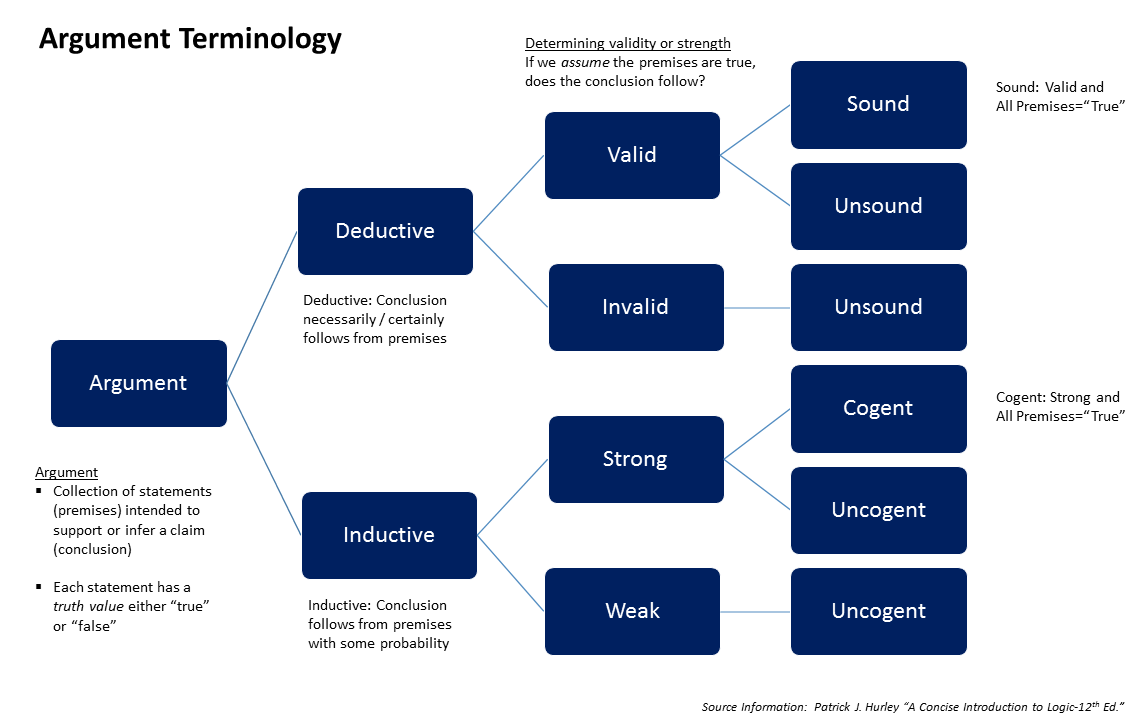
\includegraphics{argument_evaluation_chart}
\caption{A chart describing the basics of argument evaluation. Source: \url{https://commons.wikimedia.org/wiki/File:Argument_terminology_used_in_logic.png}}
\label{fig:argument_chart}
\end{figure*}

\section*{Key Terms}
\begin{fullwidth}
\begin{multicols}{2}
\begin{sortedlist}
\sortitem{Valid}{}
\sortitem{Invalid}{}
\sortitem{Sound}{}
\sortitem{Strong}{}
\sortitem{Cogent}{}
\sortitem{Deductive}{}
\sortitem{Inductive}{}
\sortitem{Fallacy}{}
\sortitem{Weak}{}
\sortitem{Confirmation bias}{}
\sortitem{Cognitive Bias}{}
\end{sortedlist}
\end{multicols}
\end{fullwidth}
